\documentclass{beamer}
\usepackage[utf8]{inputenc}

\usetheme{Madrid}
\usecolortheme{default}
\usepackage{amsmath,amssymb,amsfonts,amsthm}
\usepackage{txfonts}
\usepackage{tkz-euclide}
\usepackage{listings}
\usepackage{adjustbox}
\usepackage{array}
\usepackage{tabularx}
\usepackage{gvv}
\usepackage{lmodern}
\usepackage{circuitikz}
\usepackage{tikz}
\usepackage{graphicx}
\usepackage{longtable}
\usepackage{xparse}

\setbeamertemplate{page number in head/foot}[totalframenumber]

\usepackage{tcolorbox}
\tcbuselibrary{minted,breakable,xparse,skins}

\definecolor{bg}{gray}{0.95}
\DeclareTCBListing{mintedbox}{O{}m!O{}}{%
breakable=true,
listing engine=minted,
listing only,
minted language=#2,
minted style=default,
minted options={%
linenos,
gobble=0,
breaklines=true,
breakafter=,,
fontsize=\small,
numbersep=8pt,
#1},
boxsep=0pt,
left skip=0pt,
right skip=0pt,
left=25pt,
right=0pt,
top=3pt,
bottom=3pt,
arc=5pt,
leftrule=0pt,
rightrule=0pt,
bottomrule=2pt,
toprule=2pt,
colback=bg,
colframe=orange!70,
enhanced,
overlay={%
\begin{tcbclipinterior}
\fill[orange!20!white] (frame.south west) rectangle ([xshift=20pt]frame.north west);
\end{tcbclipinterior}},
#3,
}
\lstset{
language=C,
basicstyle=\ttfamily\small,
keywordstyle=\color{blue},
stringstyle=\color{orange},
commentstyle=\color{green!60!black},
numbers=left,
numberstyle=\tiny\color{gray},
breaklines=true,
showstringspaces=false,
}

\title
{12.472}
\date{October 9, 2025}
\author
{EE25BTECH11043 - Nishid Khandagre}

\begin{document}

\frame{\titlepage}

\begin{frame}{Question}
A rigid ball of weight 100 N is suspended with the help of a string. The ball is pulled by a horizontal force F such that the string makes an angle of 30$^\circ$ with the vertical. The magnitude of force F (in N) is
\end{frame}

\begin{frame}{Diagram}
\begin{figure}[H]
\centering
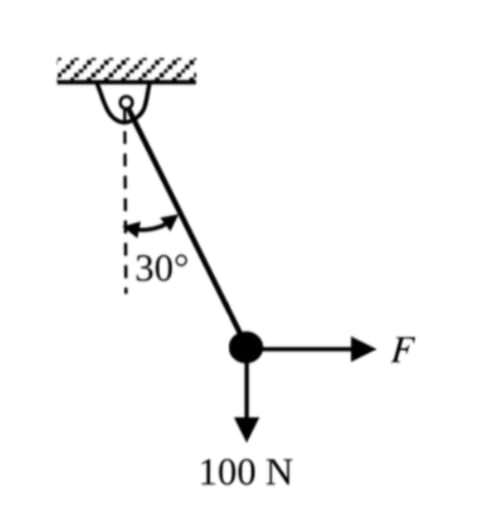
\includegraphics[width=0.4\columnwidth]{figs/fig.jpg}
\caption{1}
\label{fig:fig}
\end{figure}
\end{frame}

\begin{frame}{Theoretical Solution}
Let $T$ be the tension in the string and $F$ the horizontal force.
Equilibrium of the ball gives the linear system:
\begin{align}
T\sin 30^\circ - F = 0, \\
T\cos 30^\circ - 100 = 0.
\end{align}

\begin{align}
\frac{1}{2}T - F &= 0, \\
\frac{\sqrt3}{2}T &= 100.
\end{align}
\end{frame}

\begin{frame}{Theoretical Solution}
Writing this in matrix form $\vec{A}\vec{x}=\vec{b}$ with $\vec{x}=\myvec{T \\ F}$:
\begin{align}
\myvec{
\frac12 & -1 \\
\frac{\sqrt3}{2} & 0
}
\myvec{T \\ F}
=
\myvec{0 \\ 100}
\end{align}

Augmented matrix:
\begin{align}
\myvec{
\frac12 & -1 & \vrule & 0 \\
\frac{\sqrt3}{2} & 0 & \vrule & 100
}
\end{align}
$R_1 \rightarrow 2R_1$,$R_2 \rightarrow 2R_2$
\begin{align}
\myvec{
1 & -2 & \vrule & 0 \\
\sqrt3 & 0 & \vrule & 200
}
\end{align}
\end{frame}

\begin{frame}{Theoretical Solution}
Perform row operation $R_2 \rightarrow R_2 - \sqrt3 R_1$:
\begin{align}
\myvec{
1 & -2 & \vrule & 0 \\
0 & 2\sqrt3 & \vrule & 200
}
\end{align}

From the second row
\begin{align}
2\sqrt3 F &= 200 \\
F &= \frac{100}{\sqrt3}.
\end{align}

Thus, the magnitude of force $F$ is:
\begin{align}
F = \frac{100}{\sqrt3} \text{ N}.
\end{align}
Numerically,
$F \approx 57.7 \text{ N}$.
\end{frame}

\begin{frame}[fragile]
\frametitle{C Code}
\begin{lstlisting}
#include <math.h>

// Function to calculate the horizontal force F
// In equilibrium, summing forces in the vertical direction:
// T * cos(angle_radians) = weight
// So, Tension T = weight / cos(angle_radians)
// Summing forces in the horizontal direction:
// F = T * sin(angle_radians)
// Substitute T into the equation for F:
// F = (weight / cos(angle_radians)) * sin(angle_radians)
// F = weight * tan(angle_radians)

double calculate_horizontal_force(double weight, double angle_degrees) {
    // Convert angle from degrees to radians for trigonometric functions
    double angle_radians = angle_degrees * M_PI / 180.0;
\end{lstlisting}
\end{frame}

\begin{frame}[fragile]
\frametitle{C Code}
\begin{lstlisting}

    // F = W * tan(angle)
    double force_F = weight * tan(angle_radians);

    return force_F;
}
\end{lstlisting}
\end{frame}

\begin{frame}[fragile]
\frametitle{Python Code using C Shared Library}
\begin{lstlisting}
import ctypes

# Load the shared library
lib_code = ctypes.CDLL("./code23.so")

# Define the argument types and return type for the C function
lib_code.calculate_horizontal_force.argtypes = [
    ctypes.c_double,  # weight
    ctypes.c_double   # angle_degrees
]
lib_code.calculate_horizontal_force.restype = ctypes.c_double
# Given values from the problem
weight = 100.0  # N
angle_degrees = 30.0 # degrees
# Call the C function
force_F = lib_code.calculate_horizontal_force(weight, angle_degrees)
print(f"The magnitude of force F is (in N): {force_F:.3f}")
\end{lstlisting}
\end{frame}

\begin{frame}[fragile]
\frametitle{Pure Python Code}
\begin{lstlisting}[language=Python]
import math

def calculate_horizontal_force_pure_python(weight, angle_degrees):
    # Convert angle from degrees to radians for trigonometric functions
    
    angle_radians = math.radians(angle_degrees)

    # In equilibrium, summing forces in the vertical direction:
    # T * cos(angle_radians) = weight
    # So, Tension T = weight / cos(angle_radians)

    # Summing forces in the horizontal direction:
    # F = T * sin(angle_radians)
    # Substitute T into the equation for F:
    # F = (weight / cos(angle_radians)) * sin(angle_radians)
    # F = weight * tan(angle_radians)
\end{lstlisting}
\end{frame}

\begin{frame}[fragile]
\frametitle{Pure Python Code}
\begin{lstlisting}[language=Python]
force_F = weight * math.tan(angle_radians)
return force_F

# Given values from the problem
weight_ball = 100.0  # N
angle_string_vertical = 30.0 # degrees

# Calculate the force using the pure Python function
force_F_magnitude = calculate_horizontal_force_pure_python(weight_ball, angle_string_vertical)

print(f"The magnitude of force F is (in N): {force_F_magnitude:.3f}")
\end{lstlisting}
\end{frame}

\end{document}
